\chapter{Determination of the Luminosity Correction} \label{ch:Correction}

\section{Introduction} \label{sec:corrIntro}
The goal of the luminosity measurement experiment is to find the true measure of proton-proton collisions. The LHC sends billions of protons on a head-head collision in a collection of protons called bunches, among which only some protons collide at a given time to produce secondary particles. PLT, located at about 171 cm away from the interaction point and at rapidity, $\eta$,  of $\sim$ 4, inclusively measures the charged particles. 
%that come its way. ..count tracks to infer the number of collisions 1:1
% Ideally, one would smash two protons together many times over to figure out the cross-section. However, such experiment would take years and years to finish. Instead, billions of protons are sent on a head-head collision such that only few of them collide at a given time. This process is then repeated over and over again to get enough statistics to observe rare physics events. It is important to know that the charged particle that detector measures is actually coming from proton-proton collision and not from some secondary sources in the vicinity of detector.
%As described in chapter \ref{sec:fillScheme}, protons are made to collide in "bunches" that are separated by $25 ns$ spaced with some empty/non-colliding bunches in between. 
Within each filled bunch, the profile of the transverse density of protons is expected to be gaussian. Some protons, however, leak into neighboring bunches as seen in Figure ~\ref{fig:pBXfor}. Furthermore, protons can collide with elements within the beam pipe to produce spurious tracks. Some protons leave the ideal orbit and interact with rest gas atoms as the vacuum is not perfect, which causes secondary particle production resulting in extra tracks. 
Fig. \ref{fig:collcat} shows a schematic of tracks from several sources that can be distinguished via the track parameters--slopes, residuals. Generally, the tracks that PLT detects can be categorized as follows:

%the environment where this collision is happening also is not background free. Protons could collide with some elements within the beam pipe to produce spurious tracks, or the sub-particle from earlier bin could collide with proton from next bin, causing the secondary collisions, to produce more tracks. The goal of luminosity measurement then boils down to categorizing the events that the detector measures. Fig. \ref{fig:collcat} shows the categories of collision which can be identified via the track parameters--slopes, residuals. Generally, the tracks that PLT sees can be categorized as follows:

\begin{itemize}
    \item [1.] Tracks from IP   {\hfill + lumi}
    \item [2.] Tracks from IP with scatter  {\hfill + lumi}
    \item [3.] Tracks parallel to beam from collision with beam gas and obstructions far away from the IP    {\hfill - extra}
\end{itemize}




%At nominal beam conditions, unlike vdm, lot more bunches are filled

%Having known the conversion factor from the VdM analysis, we use the calibration constant thus evaluated to estimate the actual luminosity measured by the detectors at CMS. VdM scan is typically done with beam pairs that are separate in time. However, at the nominal luminosity of CMS, lot more collision is happening. Bunches come in 25 ns buckets in 72 trains, or 12 or single trains as described in  section \ref{fillScheme}, often producing beam halos and backgrounds that are not present during the VdM scan. As a result, data from slink cannot be saved in full BX rate, a trigger must be used to sample data at a lower rate.

%The trigger generated by taking an OR of the fast-or coincidence signals from all of the channels, run through a throttling card to keep the rate to a level that the readout could handle.




% draw collision categories
\begin{figure}[htbp!]
\centering
%\resizebox{<horizontal size>}{<vertical size>} {
%\resizebox{scale=0.8}{scale=0.8} {
	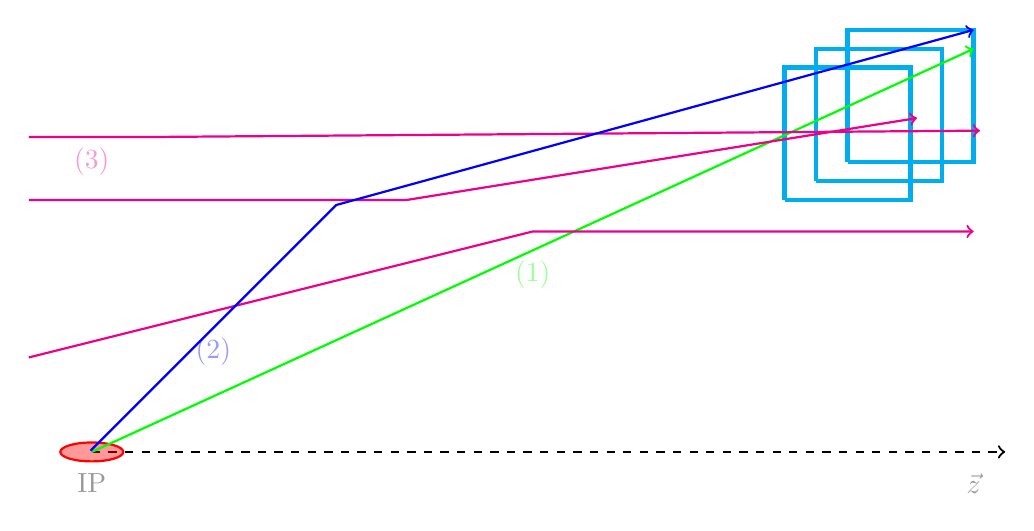
\begin{tikzpicture}[thick,fill opacity=.4,draw opacity=1,scale=0.8]
	 %three planes
	  \draw[ultra thick, cyan] (11,4) -- (13,4) -- (13,6.1) -- (11,6.1) -- (11,4);
	  \draw[ultra thick, cyan] (11.5,4.3) -- (13.5,4.3) -- (13.5,6.4) -- (11.5,6.4) -- (11.5,4.3);
	  \draw[ultra thick, cyan] (12,4.6) -- (14,4.6) -- (14,6.7) -- (12,6.7) -- (12,4.6);

	  % axes, IP
	  \draw [->, black, dashed] (0,0) --(14.5,0);
	  \node at (14,-0.5) {$\vec{z}$};
	  \draw[fill=red, red] (0,0) ellipse (0.5cm and 0.15cm);
	  \node at (0,-0.5) {IP};


	  % tracks
	  % ++ is addition to last coordinates
	  \draw [->, green] (0,0) -- node[below] {(1)} ++ (14,6.4);

	  \draw [->, magenta] (-1,5) -- node[below] {(3)} ++ (2,0) --  (14.1,5.1);
	  \draw [->, magenta] (-1,4) -- (5,4) -- (13.1,5.3);

	  \draw [->, magenta] (-1,1.5) -- (7, 3.5) -- (14,3.5);

	  \draw [->, blue] (-0.02,0.02) -- node[below] {(2)} ++ (3.9, 3.9) -- (14,6.7);

	\end{tikzpicture}
	        \captionsetup{format=hang}
	\caption{Different sources for tracks entering the PLT during proton-proton collisions. IP refers to interaction point and is the origin of genuine tracks responsible for luminosity.}
	\label{fig:collcat}
%}
\end{figure}

Two different procedures were applied for quantifying the correction term due to accidental tracks for luminosity in 2015 and 2016. Early 2015 data was compromised by the "bug" introduced during the firmware update. Algorithms used to replicate the effect in the luminosity measurement introduced by the bug will be described in section \ref{sec:firmware}, firmware issue. Procedures used to find the corrections based on track parameters for 2015 and 2016 are described in section  \ref{sec:5sigcut} and section \ref{sec:mlfit} respectively.



For the 2016 data, vdm scan data was used as a baseline to define track parameters. During vdm scan, 32 bunches are made to collide out of 3564 bunches. This means there is very small chance of the measured events to have originated from secondary collision as mentioned earlier. Section \ref{sec:mlfit} describes the theory behind the maximum likelyhood fit method used to parametrize track parameters from the vdm scan and section \ref{sec:highlumifit} provides the resulting fit to higher luminosity regime to assign a correction as a function of luminosity itself.

%move it ahead of fitting procedure?
\section{Firmware Issue} \label{sec:firmware}
%If a ROC had 3 or more hits, this would be interpreted by the FED as 0 hits which means that some of the triple coincidences were missed. The probability of getting 3 or more hits is significantly low (sub percent). To account for this issue, algorithms were written to replicate the count misses due the firmware issue using Slink data, which did not get affected by the problem. Multiple algorithms were tested, and we looked to find out the "effect" the problem had on the fast-or lumi.

%Introduced on July 31
%Fixed November 2 (between fills 4565 and fill
%4569)
%Affects a large portion of 25ns data (and the notorious fill 4246/run 254833 50ns fill)
%Two ways to measure this effect ? Transparent buffer data
%Full pixel readout (Slink)

%\subsubsection{Double Columns}

On July 31, 2015 a software bug got introduced while making a firmware update which affected how Fast-OR recognized more than 3 hits on a plane. A hit on a given plane corresponds to a charge deposit above a threshold. This charge is translated into a numerical value by the ADC in the FED. The charge deposits in every other double column are added together. Upto three levels of this signal can be distinguished to arrive at a multiplicity count inside the detector plane. The ADC value range is smaller than the dynamic range of the possible charge deposits of more than 2 hits and hence saturates. Instead of repeating the highest saturation value at high multiplicity the value was set to zero in the FED with this firmware upgrade. Hence, it reported no hit and even if the other two planes also registered at least one hit the FED would not recognize this as triple coincidence. As a result, the coincidence count underestimated by a small fraction as the likelihood for 3 hits or more on a single plane was low. To correct for this effect it was implemented algorithmically. It was decided with a counting of such cases from the ADC values obtained from a transparent buffer. 


%ADC value (which we know from gain calibration) that ought to translate to 1 coincidence count (if there was similar hit on other two planes). However, due to this bug, 3 or more hits on a single plane got translated to 0 hits. As a result, coincidence count got underestimated by a small fraction (likelihood of getting 3 hits on a plane is low) which we wanted to parametrize.

% describe what gain calibration is?

%\newcommand*{\xMin}{0}%
%\newcommand*{\xMax}{26}%
%\newcommand*{\yMin}{0}%
%\newcommand*{\yMax}{6}%
%\begin{figure}
%\centering
%\begin{tikzpicture}
%    \foreach \i in {\xMin,...,\xMax} {
%        \draw [very thin,gray] (\i,\yMin) -- (\i,\yMax)  node [below] at (\i,\yMin) {$\i$};
%    }
%    \foreach \i in {\yMin,...,\yMax} {
%        \draw [very thin,gray] (\xMin,\i) -- (\xMax,\i) node [left] at (\xMin,\i) {$\i$};
%    }
%
%\draw [step=0.5,blue, very thick] (0.25,0.25) grid (5.5,4.5);
%\draw [very thick, brown, step=0.25cm,xshift=-0.25cm, yshift=-0.25cm] (0.25,0.25) grid +(5.5,4.5);
%\end{tikzpicture}
%\end{figure}

To understand the effect of firmware issue, one has to know how FED receives signals of hits from each plane sensor. Every sensor is divided into 52 columns which is grouped into 26 double columns. Column (1,2), (3,4), (5,6) and so forth. Fast-OR records the occurrence of hits on a given double column, checks if there were hits on other two planes, and saves the result as 0/1 based on whether there was a triple-coincidence or not. The firmware undercounted the triple coincidences when one or more panels had more than 3 double columns hits for a given time period. To account for this issue, the correction was described with full pixel data. As this data contains all registered hits the expected Fast-OR rate was calculated with events that had less than 3 hits. This rate can then be compared to an accurate counts from the full pixel data to get the correction factor.

%algorithms were written to replicate the count misses due the firmware miscount using Slink data, which did not get affected by the problem. Multiple algorithms were tested, and we looked to find out the "effect" the problem had on the fast-or lumi because we don't exactly know the exact behaviour/response of detector readout under these conditions--how are pixels interpreted when adjacent columns get hit or when adjacent double columns were hit and so forth.

%Double columns
%DataHistogramsDat
%Add correction (delL/sbil) plot from transparant buffer, and algorithm replication here.
%clusters, extra clusters?

\newpage
\begin{samepage}

\begin{figure}[htbp!]
\centering
  \includegraphics[width=0.75\textwidth]%
    {figures/FastOr/firmwareRate.png}% picture filename
        \captionsetup{format=hang}
    \caption{Missing Pixel rate from Fill 4444 averaged over 5 minute interval. Missing rate from the transparant buffer is represented by $+$.}
    \label{fig:Miss_Rate}
\end{figure}

%\textcolor{red}{algo1}: count of the total number of double columns.
%
%\textcolor{green}{algo3}: count of double columns with non-adjacent columns
%
%\textcolor{yellow}{algo4}: count of double columns with non adjacent rows,columns
%
%\textcolor{blue}{algo2}: count of non-adjacent double columns


The red points(\textcolor{red}{algo1}) simply counts the number of double columns and is therefore higher than the rate from the transparent buffer. This overcounting occurs as adjacent double columns are blinded by choice of the trigger on the readout chip.
The yellow points(\textcolor{yellow}{algo4}) includes the requirement for adjacent columns on both rows and columns and is therefore lower than red and lower than the rate from the transparent buffer. This is expected as FED only checks for adjacency requirement on columns.  The green points (\textcolor{green}{algo3}) counts the number of double columns with non-adjacent columns and the blue points (\textcolor{blue}{algo2}) simply counts the number of non-adjacent double columns, both of which undershoot the rate found via the transparent buffer. This simply demonstrates that the trigger based on double columns in the readout chip does not consistently blind adjacent columns. Therefore, an average between algo1 and algo2 had to be found to match the relative rate of missing triple coincidences. This introduces some arbitrariness in the acceptance of the detector. It is included in the calibration constant $\sigma_{vis}$The rate was eventually chosen to be the one taken from the transparent buffer.

%The rate was eventually chosen to be the one taken from the transparent buffer.


%This makes sense because we know there is "some" adjacency requirement on double columns. The yellow points(\textcolor{yellow}{algo4}) checks for adjacency requirement on both rows and columns and is therefore lower than red but still lower than the rate from the transparent buffer. This also makes sense because we know there is FED only checks for adjacency requirement on columns.  The green points (\textcolor{green}{algo3}) counts the number of non-adjacent columns with non-adjacent columns and the blue points (\textcolor{blue}{algo2}) simply counts the number of non-adjacent double columns, both of which undershoot the rate found via the transparent buffer. The rate was eventually chosen to be the one taken from the transparent buffer.

\end{samepage}

%\section{Accidental Correction} \label{sec:Accidental}
%%\newpage
%Define what accidental correction means. Rename it something else?--background?



\section{Accidental Correction}

%As we dig into data to find some patterns that we can leverage for calculating the luminosity correction. The data that we save consists of all kinds of information--where did we get the hit, what time did we get the hit, at what plane, at what channel and so forth. We do know that when collision starts happening, less and less number of protons would be available for collision in succeeding cycle. We write a script to look at this data; how does the coincidence/track count vary with time?

%Of course, we cannot make every collision identical. However, as we calculate luminosity per "lumi section", we would like to know how consistent we are. How much does the luminosity change over the course of a fill? For a given lumi section, how consistent is the luminosity over bunches? Is there bunch-bunch variation? How much uncertainty/error do we have to assign for per lumi section value due to this bunch-bunch variation?

%Furthermore, from looking at the data, we see that there is fill to fill variation. How do we go about assigning uncertainty due to fill to fill variation?


%The measured luminosity from the PLT needs to be corrected for due to pure noise or random background that contribute to the luminosity or due to systematic uncertainty in the measurement itself.

There are pure noise or random track contributions to the Fast-OR counting in the PLT that need to be subtracted before translating the Fast-OR rate into luminosity as described in sec \ref{sec:lumiMeasurement}. Two different methods were used to identify such and count accidental tracks. 
Section \ref{sec:5sigcut} describes the method used in 2015 where we define accidental tracks as those that fall outside a region in the distribution of track parameters. 
The relative contribution from the sideband populations is used as relative correction to the luminosity value. 
Section \ref{sec:mlfit} describes an alternative method first applied to 2016 data that uses a maximum likelihood fit to track parameters distribution. 

%, where we establish a probability mass function for a parameter and look for deviation from the distribution to define whether any event is likely to be a "real" or fake track. As such, this method improves on the method employed in 2015.
%Using this definition, we find a percentage correction that needs to be applied to the luminosity measurement. Section \ref{sec:mlfit} describes the method used for the 2016 data, where we establish a probability mass function for a parameter and look for deviation from the distribution to define whether any event is likely to be a "real" or fake track. As such, this method improves on the method employed in 2015.



%We employed two different metrics to define what a "bad" event is for the 2015 and 2016 data. Section \ref{sec:5sigcut} describes the method used in 2015 where we define "accidental" tracks as those that fall outside certain cuts on track parameters. Using this definition, we find a percentage correction that needs to be applied to the luminosity measurement. Section \ref{sec:mlfit} describes the method used for the 2016 data, where we establish a probability mass function for a parameter and look for deviation from the distribution to define whether any event is likely to be a "real" or fake track. As such, this method improves on the method employed in 2015.

% and is used as offline correction on top of the online correction from the .



%Before discussing the correction methodology, 
%Just like any other measurement, 

%In order to know what "real" event is, we use track parameters taken from vdm scan during which beams are separated by large distance as a baseline. For the 2015 data, we look for ...


%In this section, methods used to parametrize the tracks measured by the PLT at low luminosity regime, and the subsequent fit to high lumi regime will be discussed. 
%
% FIT AT VDM
%
%We use vdm scan to understand the shape of our beams and get a conversion factor for the luminosity measurement. As we scan the beams across each other, the overlap between beams changes and thus the number of proton-proton collision also changes. We then make a fit for the number of tracks as a function of beam separation to get the conversion factor at no separation between beams.

%The proton-proton collision at nominal separation gives us the conversion factor which basically tells use the expected number of collision at 0mm beam separation. Unlike vdm scans where neighboring bunches are well separated, a set of continuous bunches are typically filled at nominal beam conditions. This introduces few complications with our conversion factor extracted from vdm analysis which needs to be corrected for. As we increase the number of filled bunches and as we increase the single bunch instantaneous luminosity (SBIL), we would like to understand how the number of collision, thus luminosity, changes.

%Ideally, if per bunch luminosity was the same and only the number of filled bunch were to change, we can just multiply the number of bunches by conversion factor from vdm scan to get the new expected luminosity. This is not the case, however. Firstly, lot more bunches are filled and most bunches come into "trains"--a set of continuous filled bunches. Even though $\sim10^{11}$ protons are supposed to be confined within a $25 ns$, some protons manage to leak to bins ahead and behind the supposed bin. This creates "beam halos" which needs to be accounted for. Furthermore, luminosity per bunch i.e. SBIL also increases at regular fills. Both these new factors contribute differently to the luminosity that we measure via our telescopes.


%pdf at vdm


\subsection{Track Parameters} \label{sec:trackparams}

PLT is positioned so that it accepts tracks that originated at the IP coming at particular angle. Background tracks are less likely to pass through all three planes of the telescope because of the way plane 0, 1, and 2 are positioned. Still, stray protons could collide with other stray protons to produce secondary particles that pass though all planes of a telescope which can be mistaken for genuine tracks. Sub-particles could also collide with instruments/molecules in the tube to make fake tracks. 

The slope-y of all tracks is expected to be a distribution with mean close to the telescope's slope against IP and slope-x mean is expected to be close to 0. The goal is to look at the data and see how track parameters change with respect to the these parameters from the vdm scan where beams were far separated, and SBIL was close to 0.


\subsubsection{Track parameters at VdM}
Beam conditions for vdM are different than the regular nominal physics operation, with lower beam intensities and large separation between few dozens of filled bunches. As such, contribution from background is expected to be lower, esp since trigger is only set for colliding bunches. Figure \ref{fig:vdm54} shows the number of tracks as a function of beam separation during the "Y1 scan" in 0.5 $\sigma$ steps. Special trigger was employed for vdm scan to collect as many tracks as possible. 32 colliding bunches, and 5 con-colliding bunches were triggered for Fill 4954. 
%Tracks from vdm scan at $0mm$ separation were investigated to find the PDF of slope x and slope y. 


%we expect to see collision measurement coming from beam halos or other background factors which we would like to calculate and account for. 


%For VdM Scan, special trigger was employed. Fig. \ref{fig:vdm54} shows the track rate for "Y1 scan". Beams are separated in 0.5 $\sigma$ steps.

\begin{figure}[htbp!]
\centering
  \includegraphics[width=0.8\textwidth]%
    {figures/VdM/VdMFill.png}% picture filename
        \captionsetup{format=hang}
    \caption{Number of tracks vs Beam separation, VdM Fill 4954(2016)}
     \label{fig:vdm54}
\end{figure}

At higher luminosities when trigger is random and the per instantaneous luminosity is higher, however, non-luminosity contributions as explained in \ref{sec:corrIntro} are expected to increase. The goal is to find this extra contribution to luminosity measurement as a function of luminosity itself. Probability mass function of track parameters slope-x and slope-y was constructed using 50566 tracks reconstructed by applying the triple-hit condition for the $0$ mm separation of beams during VdM separation scan(Y1). Afterwards, deviations from the distributions at higher luminosity was investigated to find out the extra tracks that is seen beyond what is seen at vdm. 


\subsection{5 Sigma Cut Procedure} \label{sec:5sigcut}
For the 2015 run period, fill 4444 was chosen as a representative fill where PLT had the least operational issues. Uncertainty to luminosity was assigned by making quality cuts to track parameters. As shown in Figure \ref{fig:44Slope_Y}, a Gaussian was fitted to slopes and residuals, and  tracks falling outside the cut boundaries were investigated. 

%any tracks outside 5 sigma from the mean is treated as a 'bad' track. Uncertainty from the change in cut is taken into account 

%5 sigma cuts applied to slopes and residuals to get a linear relationship between the accidentals and the SBIL.


\begin{figure}[htbp!]
\centering
  % trim = {<left> <lower> <right> <upper>}
  \includegraphics[width=0.7\textwidth, trim = {0.2cm 0.2cm 0.2cm 0.25cm}, clip]%
    {figures/slink/Fill4444_SlopeY_SigmaCuts.png}% picture filename
        \captionsetup{format=hang}
    \caption{Slope-y from Fill 4444 with sigma cut boundaries}
    \label{fig:44Slope_Y}
\end{figure}

It was found that applying cuts outside $4.5$ to $5 \sigma$ and $5$ to $5.5 \sigma$ had little impact on the accidental correction. A combined cut of $5 \sigma$ was applied to both slopes and residuals to define a bad track. Table \ref{tbl:accCorr} shows the various cuts applied to slopes and residuals. Uncertainty of 1.5 \% is assigned to accidental definition resulting from change in cut criteria.

\begin{table}[htp]
\begin{center}
\begin{tabular}{| c | c | c | c | c |}
\hline
$\vert S_{x} \vert$ cut & $\vert S_{y} - S_{PLT} \vert $ cut & $R_{x}$ cut (cm) & $R_{y}$ cut (cm) & Measured Accidental Rate \\ \hline
0.002 & 0.007 & 0.03 & 0.03 & 11 \% \\ \hline
0.03 & 0.0105 & 0.03 & 0.03 & 8 \% \\ \hline
0.03 & 0.0105 & 0.02 & 0.02 & 10\% \\ \hline
\end{tabular}
\end{center}
    \captionsetup{format=hang}
\caption{Variation in the measured accidental rate with different sets of cuts in track parameters.}
\label{tbl:accCorr}
\end{table}%



%\subsection{Consistency of relative-luminosity measurements during physics running}


%\section{VdM} \label{ch:vdm}
%\newpage
\subsection{Maximum Likelihood Fits} \label{sec:mlfit}

Suppose that we have a sample of some n number of independent observations $x_{1}, x_{2}, ..., x_{n}$ from a theoretical distribution $f(x | \theta)$ where $\theta$ is the parameter we would like to find. Let $f(x_{1} | \theta)$ be the probability of observing $x_{1}$ data given $theta$ parameter for function $f$. Then, the probability of observing $x_{1}, x_{2},...,x_{n}$ data is given by the \emph{likelihood} function

\begin{equation}
L(\theta | x) = f(x_{1} | \theta) f(x_{2} | \theta) \cdot \cdot \cdot f(x_{n} | \theta)
\end{equation}

Since we have $x_{1}, x_{2},...,x_{n}$ data and we would like to know what $\theta$ is, L is maximized by 
$$
\frac{dL}{d\theta} = 0
$$

For distributions of the exponential nature, maximum of  the logarithm of L can be found via
$$
\frac{d(lnL)}{d\theta} = 0
$$
The solution to $\hat{\theta}$ is the maximum likelihood $estimator$ for parameter $\theta$ for a given sample. For other samples, $\hat{\theta}$ could be different and thus  $\hat{\theta}$ is a probability distribution. The standard deviation on  $\hat{\theta}$ gives the size of the error in our estimation for true  $\theta$.



%Bin widths are chosen to be smaller than the experimental resolution.

\subsubsection{Likelyhood Fit of slope-x at vdm}

The alignment of telescopes is such that there is no preference for slopes to have a particular slope in x-direction, if a track truly originates from the interaction point.

$$
VdM \textunderscore X = {\color {cyan}Gaussian_{core}(\sigma_{1}, \mu_{1})} + f_{1}* {\color {green} Gaussian_{outlier}(\mu_{2},\sigma_{2})}
+ f_{2} * {\color {red} Gaussian(\mu_{3},\sigma_{3})}
$$


\begin{figure}[htbp!]
\centering
  \includegraphics[width=0.7\textwidth]%
    {figures/VdM/VdMSlopeXModel.png}% picture filename
        \captionsetup{format=hang}
            \captionsetup{format=hang}
    \caption{SlopeX model using reconstructed tracks from vdm scan at nominal separation}
    \label{fig:VdM_Xmodel}
\end{figure}

Fig \ref{fig:VdM_Xmodel} shows the model used for the $x$-slope of the tracks during VdM Y1 scan Fill 4954. Main signal is dominated by a core Gaussian (red), a broader gaussian (green) and yet another gaussian (dashed blue) that spans the range of $x$-slope. The mean value for all the pdfs is close to zero, which is due to the fact that there is no reason for a track to have any preference in the $x-y$ plane.

% group slope-x and slope-y together?

\subsubsection{Likelyhood Fit of slope-y at vdm}

Middle plane for each telescope is placed 0.102 cm higher(lower) than first(third) plane. Since the length of telescope is 7.5 cm, the $y$-slope of telescope itself is around 0.027 which is what $y$-slopes of tracks is expected to be on average.

\begin{figure}[htbp!]
\centering
  \includegraphics[width=0.6\textwidth]%
    {figures/VdM/VdMSlopeYModel.png}% picture filename
        \captionsetup{format=hang}
    \caption{SlopeY model using reconstructed tracks from vdm scan at nominal separation}
    \label{fig:VdM_Ymodel}
\end{figure}


Fig \ref{fig:VdM_Ymodel} shows the 3 gaussian fit to the slope-$y$ data from VdM Fill Y1 scan. Main signal is dominated by the core gaussian centered at around $0.027$, another gaussian, and one bifircated gaussian with large $\sigma_{1}$ and $\sigma _{2}$. 

$$
VdM \textunderscore Y = {\color {cyan}Gaussian_{core}(\sigma_{1}, \mu_{1})} + f_{1}* {\color {green} Gaussian_{outlier}(\mu_{2},\sigma_{2})}
+ f_{2} * {\color {red} BiGaussian(\mu_{3},\sigma_{31},\sigma_{32})}
$$





\subsubsection{Combined Fit}
A combined model is constructed using the parameters fixed for both slope-$x$ and slope-$y$ with a extra pdf on top of vdm-$x$ and vdm-$y$ models. The extra contribution to the pdf is allowed to float with a common fraction f for both slopes. Figure \ref{fig:combinedModel} shows the combined fit to one sample data from a regular fill. Both slope-$x$ and slope-$y$ have a predefined shape of signal taken from the individual fits to slope-$x$ and slope-$y$.

%Both slope-x and slope-y parameters are fed into a model and asked to fit to the VdM data. Ideally, this should produce the null result which is what we find. We then use the parameters and add extra pdf on top of slope-x and slope-y models separately.



$$
Combined \textunderscore Fit = \left ( {\color {green}VdM\char`_X} + f* {\color {magenta} Extra \textunderscore x} \right ) \times \left( {\color {green}VdM\char`_Y} + f* {\color {magenta} Extra \textunderscore y} \right)
$$

\subsection{Fit Validation}
For each individual fit to slopes, different distributions were tested, including gaussian, polynomials, and double-gaussians. For slope-$x$, for instance, a double gaussian eventually converged back to a gaussian. 

As mentioned earlier, there were 50566 reconstructed tracks from the vdm scan. Some of these tracks, however, came from the non-colliding bunches (5 out of 37 triggered bunches were colliding bunches). Same fit was done for tracks from colliding and non-colliding bunches separately and it was found that there was not much difference in the fit parameters with the changes. 

%Probability mass function
%For each fit to slopes, each PDF was chosen after careful 
%
%The combined model was then fitted to the reconstructed tracks from vdm which assigned 0 fraction to the "extra" stuff which gave a confirmation of the combined model. Furthermore, fitting the model to tracks from only the colliding bunches also gave fraction 0.
%
%separated colliding and non-colliding bunches and made a fit. Didn't change much.
%tweaked gaussians ==> converged to earlier.
%monte carlo simulation







\section{Results} \label{sec:highlumifit}

\begin{figure}[htbp!]
  \includegraphics[width=1.0\textwidth]%
    {figures/VdM/CombinedFit_II.png}% picture filename
    \caption{Combined Fit to the Model}
    \label{fig:combinedModel}
\end{figure}

The combined model is then fitted to reconstructed tracks from regular fills at higher luminosities.  A bifurcated gaussian is used as an extra pdf for slope-$y$, and a regular gaussian was used as an extra pdf on top of slope-$x$ model. Figure \ref{fig:correction} shows the increase in the area under the magenta curve as a function of SBIL. The blue line, 2.2\% + SBIL * 1.4\%, is from correction to 2015 data where $5 \sigma$ cut was applied to slopes and residuals. The black dots which increase with a slope of $0.82$ as a function of SBIL, is from 2016 data where likelihood fit method was applied. Fitted line to the black dots goes all the way back to 0, which is the vdm scan with very low value for SBIL. The dotted lines around the black dots represent the uncertainty in the frac3. 

%Since slope from likelihood fit grows slower




%\section{Results}


\begin{figure}
\centering
  % trim = {<left> <lower> <right> <upper>}
  \includegraphics[width=0.8\textwidth, trim = {2.5cm 7.2cm 2.5cm 5cm}, clip]%
    {figures/VdM/correction.pdf}% picture filename
    \captionsetup{format=hang}
    \caption{Coorection as a function of Single Bunch Instantaneous Luminosity (SBIL). The dashed line correspond to the error bars in fraction of non-lumi contribution.}
    \label{fig:correction}
\end{figure}


%colliding bunches only to understand the sensitivity of combined model 
%if the combined fit assigns some fraction f. This made almost no difference i.e. the combined model agrees with the 



%\subsubsection{Residuals}
%
%% describe what residuals mean
%
%\begin{figure}[htbp!]
%\centering
%  % trim = {<left> <lower> <right> <upper>}
%  \includegraphics[width=0.8\textwidth, trim = {0cm 12cm 23cm 0cm}, clip]%
%%  \includegraphics[width=0.7\textwidth]%
%    {figures/VdM/resSample.png}% picture filename
%    \caption{Sample residual distribution for slope-y from combined fit}
%    \label{fig:Res_Ymodel}
%\end{figure}
%
%
%\subsection{Systematics}
%For each slopes, several pdfs were used with floating fraction. The pdf for slope-x and slope-y that we used finally was found to be the most significant.
%
%\begin{itemize}
%\item Validate fit with Toys
%\item cross check: fit VdM ddata with full model $\rightarrow$  fits $f = 0$
%\item systematic uncertainty - shape variation
%\item try two gaussians with well separated mean (and sigma) instead of single gaussian --when floated coverges back to single gaussian(bigaussian)
%\item single gaussian and bigaussian interchanged
%\item fix widths to values of measurements at comparable luminosity
%\item Let VdM core Gaussian parameters float
%\end{itemize}


\subsection{Toy Monte Carlo Simulation}

A monte-carlo toy simulation was performed to understand the relationship between the accidental cut applied for 2016 data and the fraction of magenta curve from the likelihood fit. For a sample Fill, 100,000 tracks were generated with parameters from the combined model and the fraction of magenta was fixed to some value. A single gaussian was fitted to slope-$x$ and slope-$y$ separately, and the sigma and mean was extracted. Afterwards, the number of tracks falling outside the 5$\sigma$ cut on slope-$x$ and slope-$y$ was calculated multiple times for a given fraction3. The result is shown in figure \ref{fig:montecarlo} and it shows a linear relationship between the area under the magenta curve and the 5 sigma cut. The slope from the fit is 0.82, and the intercept is 7.63. Slope less than 1 implies that the area under magenta curve increases faster than the area outside the 5 sigma cut.
%The slope of $0.82$ implies that the area under magenta curve grows faster than the area under the 5 sigma cut.


\begin{figure}[htbp!]
\centering
  % trim = {<left> <lower> <right> <upper>}
  \includegraphics[width=1.0\textwidth, trim = {1cm 2.5cm 1cm 1.5cm}, clip]%
%  \includegraphics[width=1.0\textwidth]%
    {figures/VdM/mc.png}% picture filename
        \captionsetup{format=hang}
%    \caption{Fit model reconstruction of tracks outside $5 \sigma$}
\caption{Extrapolation of fit model to high accidental fractions vs the counting of the track in tails (outside $5 \sigma$) variable distributions.}
    \label{fig:montecarlo}
\end{figure}

It should be noted that the 5 sigma cut applied for 2015 data was on both the slopes and residuals.  Maximum likelihood fit was done for the relevant independent variables, the slopes, and residuals are simply taken as a measure of track quality. A correction was then applied to the 5 sigma cut procedure that was applied for 2015 data. 
%In effect, this correction is for the contribution to correction for 2015 data from bad slopes. Keeping the 5 sigma cut from residuals as a check on track quality, one can apply 18\% correction to 2015 accidental correction. Instead, if residuals were to be taken out of the equation, one has to look at the result from accidental correction using 2015 procedure and likelihood fit procedure. This was done for a representative fill and the slope was $1.23$, meaning that the area under magenta curve grew slower than the 5 sigma cut.





%Correction on top of 5 sigma cuts
%\section{Luminosity Correction}

%\begin{table}[htp]
%\begin{center}
%\begin{tabular}{|r|c|}
%    \hline
%
%Systematic source & Systematic uncertainty[\%] \\    \hline
%
%Absolute calibration from VdM scan & 2.6 \\     \hline
%
%\end{tabular}
%\end{center}
%    \captionsetup{format=hang}
%\caption{Systematic uncertainties on the PLT luminosity measurement for the Year $25ns$ run.}
%\label{default}
%\end{table}%




%\begin{table}
%\begin{center}
%    \begin{tabular}{| l | l | l | l |}
%    \hline
%    {\bf Interaction} & {\bf Strength} & {\bf Theory} & {\bf Mediator} \\ \hline
%    Strong & 10 & Quantum Chromodynamics & Gluon \\ \hline
%    Electromagnetic & $10^{-2}$ & Quantum Electrodynamics & Photon \\ \hline
%    Weak & $10^{-3}$ & Flavordynamics &  W and Z Bosons\\ \hline
%    Gravitation & $10^{-42}$ & Geometrodynamics & Graviton \\
%    \hline
%    \end{tabular}
%     \caption{Rough order of the interaction strengths, the mediator and the theory, which describes
%these interactions}
%
%\end{center}
%\end{table}


\section{Conclusion}
%The search for and detailed study of new particles and forces with the Compact Muon Solenoid (CMS) detector at the Large Hadron Collider (LHC) of CERN is fundamentally dependent on the precise measurement of the rate at which proton-proton collisions produce any particles, the so-called luminosity. 
%Therefore, a new detector, the Pixel Luminosity Telescope (PLT), dedicated to measure the luminosity at high precision was added to the CMS experiment in 2015.
%It measures the inclusive charged particle production from each collision of proton bunches in the LHC. The instrument provides measurements of particle trajectories which allows to distinguish particles originating from proton proton collisions and other sources that accidentally are created as luminosity contribution.
%Methods were developed to calculate the corrections to the luminosity measurement of the PLT.

I built data pipelines for real-time data visualization and monitoring, wrote alarm system for anomalies detection by inspecting time-series data. I also wrote codes to make event reconstruction, analysis code to make statistical models for classification and prediction of  signal and background events in data sets.

Correction to the luminosity measurement by the Pixel Luminosity Telescope (PLT) for the CMS experiment at the Large Hadron Collider was calculated for 2015 and 2016 run period using data-driven statistical methods. Result from likelihood fits were used to improve the background subtraction from non luminosity contributions.

% 0.82 from slope ==> some of the .18 can be attributed to either residual contribution.
% However, from data, we see a different slope.
